%%%%%%%%%%%%%%%%%%%%%%%%%%%%%%%%%%%%%%%%%%%%%%%%%%%%%%%%%%%%%%%%%%%%%%%%%%%%%%%%
%%%%%%%%%%%%%%%%%%%%%%%%%%%%% IMPORTS AND SETTINGS %%%%%%%%%%%%%%%%%%%%%%%%%%%%%
%%%%%%%%%%%%%%%%%%%%%%%%%%%%%%%%%%%%%%%%%%%%%%%%%%%%%%%%%%%%%%%%%%%%%%%%%%%%%%%%

% General settings
\documentclass[11pt,a4paper,notitlepage]{article}

% Misc includes
\usepackage{array}
\usepackage{xcolor}
\usepackage{longtable}

% For title + abstract page
\usepackage{titling}

% For table of contents with links
\usepackage{hyperref}
\hypersetup
{
    colorlinks,
    citecolor=black,
    filecolor=black,
    linkcolor=black,
    urlcolor=blue
}
\usepackage{ulem}

% For images
\usepackage{graphicx}
\usepackage{subfig}

% For quotes
\usepackage[english]{babel}
\usepackage[autostyle, english = american]{csquotes}
\MakeOuterQuote{"}

% For including code
\usepackage{listings}
\usepackage{color}
\definecolor{dkgreen}{rgb}{0,0.6,0}
\definecolor{gray}{rgb}{0.5,0.5,0.5}
\definecolor{mauve}{rgb}{0.58,0,0.82}
\lstset{
  language=Java,
  aboveskip=3mm,
  belowskip=3mm,
  showstringspaces=false,
  columns=flexible,
  basicstyle={\small\ttfamily},
  numbers=none,
  numberstyle=\tiny\color{gray},
  keywordstyle=\color{blue},
  commentstyle=\color{dkgreen},
  stringstyle=\color{mauve},
  breaklines=true,
  breakatwhitespace=true,
  tabsize=3,
  %frame=single,
  rulesepcolor=\color{gray},
  rulecolor=\color{black}
}

% Math
\usepackage{amssymb,amsmath}
\setlength{\thinmuskip}{3\thinmuskip}
\setlength{\medmuskip}{3\medmuskip}
\setlength{\thickmuskip}{3\thickmuskip}

% Document title data
\title{\Large{TODO\\2015-2016}\\\Huge{TODO}}
\author{836897 Simone Graziussi}
\date{TODO}



%%%%%%%%%%%%%%%%%%%%%%%%%%%%%%%%%%%%%%%%%%%%%%%%%%%%%%%%%%%%%%%%%%%%%%%%%%%%%%%%
%%%%%%%%%%%%%%%%%%%%%%%%%%%%%%%% DOCUMENT START %%%%%%%%%%%%%%%%%%%%%%%%%%%%%%%%
%%%%%%%%%%%%%%%%%%%%%%%%%%%%%%%%%%%%%%%%%%%%%%%%%%%%%%%%%%%%%%%%%%%%%%%%%%%%%%%%

\begin{document}

\sloppy

%............................................................................%
%................................ TITLE PAGE ................................%
%............................................................................%

\begin{titlingpage}
    \maketitle
    \begin{abstract}
        \large{TODO}
    \end{abstract}
\end{titlingpage}


%..............................................................................%
%............................. TABLE OF CONTENTS ..............................%
%..............................................................................%

\newpage
\tableofcontents
\newpage


%..............................................................................%
%................................... INTRO ....................................%
%..............................................................................%

\part{Introduction}

\section{Abstract}

\section{Testing}
Testing is the process used in software development to assess the validity of functional and non-functional requirements of an application. Although this verification is able to guarantee the correctness of the tested components within the specific conditions described by the test cases, testing cannot assess the validity of the whole application in every situation, because this would require an unfeasible amount of detail. For this reason, testing is mainly used to discover software bugs in particular situations and to reach an acceptable confidence that the program works as expected under the most common conditions.\bigskip \\
Test cases require a mechanism to actually determine the test outcome, i.e. to tell if the application behaves as expected during the validation process. This mechanism, called oracle, should ideally be complete but avoiding over-specification, while also being efficiently checkable~\cite{Baresi:Oracles}. Oracles can assume many forms, for example the behavior of the application is compared with the technical specifications (e.g. documentation), it is automatically checked by the system thanks to some constructs that allow the developer to specify the test conditions or it can even be manually evaluated by a human being.\bigskip \\
Test cases can be designed from different points of view. In particular, we can have:
\begin{itemize}
	\item White-box testing: the focus is on the internal structure of the application, i.e. tests are defined at the source code level (\textit{how} the software behaves).
	\item Black-box testing: examines the external behavior of the application without considering the actual implementation, i.e. tests are defined at the user level (\textit{what} the software does).
	\item Grey-box testing: combination of white-box and black-box testing. Tests are defined with a partial knowledge of the internal structure of the application (i.e. how the main components interact and the general algorithms used).
\end{itemize}\bigskip
There are usually four levels on which test cases can be defined:
\begin{itemize}
	\item Unit Testing: focuses on a specific unit of the program, for example a single function/method/class used in the source code. Usually, it follows a white-box testing approach and it is performed during development to build a program using units guaranteed to work.
	\item Integration Testing: tests interactions between components of the application, i.e. it usually puts together the units tested in the previous step to see if they work well together.
	\item System Testing: it considers the program as a whole to see if it meets all requirements and quality standards.
	\item Acceptance Testing: final step that decides if the application is complete and ready to be deployed (e.g. released to the public)
\end{itemize}

\section{Android}
Android is a operating system (OS) developed by Google. It is designed primarily for touchscreen mobile devices like smartphones and tablets, but recently it was extended to televisions (Android TV), cars (Android Auto) and smartwatches (Android Wear).\medskip \\
The OS is a multi-user Linux system in which each app is a different user. It is characterized by the so called sandboxing mechanism: each process runs in its own virtual machine (VM) and so every app runs in isolation from the other applications. This means that, by default, an application can access only a limited set of components and cannot access parts of the system for which it does not have permissions.\medskip \\
Android applications are developed in a Java language environment. The Android Software Development Kit (SDK) compiles code, data and resources into a package called APK, which is used by the devices to install the application.

\section{Android App Components}
Android applications are built by five main components, each with its specific purpose:
\begin{itemize}
	\item Activity: an activity represents a single "action" that the user can take and, since almost all activities interact with the user, they provide a screen with a user interface. Each activity in the application is independent from the others, but it is of course possible to start an activity (for example when the user clicks on a button) from another to build the application flow.
	\item Fragment: this component was introduced in Android 3.0 (API level 11) to support dynamic and flexible UI on large screens, for example on tablets. A Fragment  represents a "portion" of an Activity, with its own state and UI. Each Activity can contain multiple Fragments at a time, Fragments can be added/removed at runtime and each Fragment can be reused in more than one Activity. A Fragment can only be instantiated inside an Activity.
	\item Service: a service is a component that is executed in background and, as such, it provides no user interface. It is used to perform complex computations or to interact with an external API (e.g. via the network). The advantage of this approach is that another component (e.g. an Activity) can start and interact with a Service in order to avoid blocking its UI with computationally intensive operations.
	\item Content Provider: a content provider allows to store and retrieve data in some persistent storage location, for example a local SQL database or a remote repository. The provided data can be shared among different applications or private to a specific one.
	\item Broadcast Receiver: a broadcast receiver responds to global messages, i.e. messages received by all applications on the device. These events may be fired by the system (e.g. the device has just rebooted) or by a single application (e.g. some data is available), and then intercepted by the applications interested to them.
\end{itemize} 
Activities, services and Broadcast Receivers are started asynchronously by messages called Intents. This allows not only an application to start its own components, but also to call on other applications. For example, a game may start its internal GameService to manage the game loop, but also send an intent to a social network application to share the game progress.

%..............................................................................%
%............................ STATE OF THE ART ................................%
%..............................................................................%

\part{Android Testing State of the Art}

Android tests are mainly based on JUnit~\cite{JUnit}, a testing framework for Java. It allows to create classes called test cases that contain methods annotated with \texttt{@Test}, each representing a test.

\section{Unit Testing}
White-box unit testing in Android can be
\begin{itemize}
	\item Local: it runs on the local development machine (i.e. the computer where the application is coded). It has the advantage of being fast (avoids the overhead to load the application in a device/emulator), but can be exploited only if the tested unit has no dependencies or simple dependencies. This means that the test case should not use any device-specific features (e.g. expect a sensor input) or, if it does so, they should be minimal since they need to be mocked using for example tools like Mockito~\cite{Mockito}.
	\item Instrumented: it is executed in a physical device or on an emulator and so has access to instrumentation information, such as the Context (information about the application environment). It is slower than the previous case but it's more convenient if the unit dependencies are too complex to mock.
	\item Hybrid: the external library Robolectric~\cite{Robolectric} tries to take the advantages of the previous two approaches, i.e. it runs "instrumented" tests on the local machine, without mocking. As reported on the website, Robolectric allows a test style that is closer to black box testing, making the tests more effective for refactoring and allowing the tests to focus on the behavior of the application instead of the implementation of Android.
\end{itemize}

\section{UI Testing}
Android also provides a way to test User Interface (UI) to see if it behaves as expected. This type of testing can be defined as a grey-box approach: the application is tested at the user level without considering the actual implementation of the UI, but the definition of the test cases may require to know some information on the internal structure, for example the IDs of the buttons to be clicked.
\begin{itemize}
	\item UI testing on a single app: the Espresso library provides APIs for writing UI tests to simulate user interactions. In general, defining a test case means building a series of \texttt{onView(Matcher).perform(ViewAction).check(ViewAssertion)} instructions, i.e. select a particular View that matches some description (e.g. a button with "Start" text), perform one or more actions on it (e.g. click) and check if some conditions are true (e.g. if after the click the button text changes). The main advantages of Espresso are that the test cases are easily readable and understood, and that it has automatic synchronization (before performing an action it waits for the previous ones to be completed, i.e. for the main thread to be idle).
	\item UI testing on multiple apps: the UI Automator library allows to test if the developed application interacts correctly with the system or other apps (e.g. the application may request an image, the Camera app is opened, the picture is taken and then the control goes back to the original application). 
\end{itemize}

\section{Runner Tools}
In addition to the testing frameworks described in the previous sections, Android also offers some tools to run and test an application without accessing the source code (black-box testing):
\begin{itemize}
	\item UI Exerciser Monkey: allows to run an application on a physical device or emulator generating a pseudo-random (but repeatable) streams of user events (e.g. clicks) and system-level events (e.g. start call). The developer can set several options like target package, probability of certain events, etc.
	\item monkeyrunner: controls a device or emulator from a workstation by sending specific commands and events defined as a Python program. It also allows to take screenshot during the test execution and store them on the workstation.
\end{itemize}

\section{Assertions in Android}
An assertion is a statement at a specific point in a program that enables to check an assumption. It is expected to be true, but if a bug is present the assertion will fail and the system will throw an error. Assertions are test oracles that specify what the application does rather than how.
\bigskip \\
In Java, the assertion statement is
\begin{lstlisting}
assert Expression1 : Expression2;
\end{lstlisting}
where \texttt{Expression1} is the boolean expression to be checked and \texttt{Expression2} is an expression that has a value to better describe the error. If \texttt{Expression1} is false, an \texttt{AssertionError} exception is thrown.\bigskip \\
Many frameworks, including JUnit itself, offer several utility methods to easily write more complex assertions without using the \texttt{assert} keyword. For example, the method \texttt{assertEquals(String message, Object expected, Object actual)} checks that the two given objects are equal and, if not, throws an \texttt{AssertionError} with the given message.\bigskip \\
Since Android has its own virtual machine ART, which is not compatible with JVM from Oracle, the \texttt{assert} keyword is not supported by default\footnote{It is however possible to manually enable assertions on a given device using for example the Android Debug Bridge command \texttt{adb shell setprop debug.assert 1} (assertions will be enabled for all applications until the device is rebooted), but the Android developers themselves discourage their use}. For this reason, in an Android application assertions are usually created exploiting JUnit-like methods that directly throw an \texttt{AssertionError} if the check fails. This means for example using the assertions provided by Android (via \texttt{Assert}, \texttt{MoreAsserts} and \texttt{ViewAssert} classes), the JUnit framework itself or other external libraries.

\section{What's missing in Android testing (?)}
?

%..............................................................................%
%............................... BACKGROUND ...................................%
%..............................................................................%

\part{Background}

\section{Introduction to Events}

\section{Background/Motivation}

\section{Three Levels of Testing}


%..............................................................................%
%.................................. LIFECYCLE .................................%
%..............................................................................%

\part{Lifecycle Testing}

\section{Introduction}
The focus this part of the thesis is on a specific type of events that are generated by Android applications: lifecycle changes. As it will be explained later in detail, handling the lifecycle of the app components like Activities and Fragments is a critical aspect of Android development, and so this type of events deserves a separate in-depth analysis.\medskip \\
In particular, two approaches for lifecycle testing will be proposed: static analysis and dynamic analysis. The former will try to analyze the source code of the application to detect possible issues related to the handling of some components in accordance to the host Activity/Fragment lifecycle, for example failing to release a resource that was previously acquired. The dynamic analysis approach, instead, will focus on pre-generated test cases that allow the developer to express some actions to be performed and conditions to be checked in common lifecycle events sequences, which will be used in several tests to assess the robustness of the application.\medskip \\
The following sections will present first a detailed explanation of the main concepts of lifecycle in Android applications, then the static approach will be analyzed and finally the dynamic approach will be described.

\section{Lifecycle}

\subsection{Component Lifecycle}
App components in Android such as Activities, Fragments and Services are characterized by their lifecycle, i.e. the current runtime state. In general each component is started and then destroyed, but some can also be paused and resumed, and go through several other states. When a lifecycle state transition happens, the Android system allows the developers to implement some callbacks (Java methods, usually overridden from the component class) in the component implementation to manage their behavior in those particular situations.

\subsection{Activity Lifecycle}
An Activity can be in three static states:
\begin{itemize}
	\item Resumed: the Activity is visible and can receive user input
	\item Paused: the Activity is \textit{partially} hidden by another visual component, for example a notification dialog, and has lost the focus. When the activity is paused it cannot receive any user input o execute code.
	\item Stopped: the Activity is completely hidden to the user, i.e. it is in the background. Like in the previous case, the activity cannot receive inputs or run code. In this state the Activity is still "alive": the state (e.g. member variables) is retained and the Activity can be later restarted.
\end{itemize}
An Activity can also be in two transient states:
\begin{itemize}
	\item Created: the Activity has been instantiated and will soon become Started
	\item Started: the Activity has been initialized and will soon become Resumed
\end{itemize}
Finally, an Activity can be Destroyed. In this "state" the Activity instance is dead. An Activity can for example be destroyed by the OS when it is stopped and the device needs to free resources.\bigskip \\

The Activity class provides several callbacks for lifecycle changes. These methods can be implemented by the developer to manage the state of the Activity: for example \texttt{onCreate()} can be used to initialize the UI components, \texttt{onStop()} to free resources for the other applications. Note that not all callbacks need to be explicitly implemented for each activity: actually simple Activities usually implement only \texttt{onCreate()}.\bigskip \\

This image shows a simplified scheme of the Activity lifecycle transitions with the corresponding callbacks.
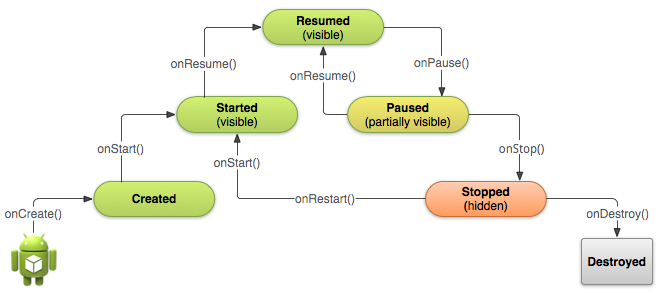
\includegraphics[width=450px]{Images/Android/basic-lifecycle.png}

[TODO extend with more detailed explanations of callbacks, save instance, etc.? More detailed diagram?]

\subsection{Fragment Lifecycle}
The lifecycle of a Fragment is closely related to the lifecycle of the Activity that contains it: for example, when an activity is paused, all the contained Fragments are paused too. In addition to this, however, Fragments can go through lifecycle changes independently of their host Activity: in particular, since fragments can be dynamically added and removed at runtime, they can be created and destroyed while the Activity is running. Moreover, the developer also has the option to store removed fragments in the so-called backstack and be able to restore them later for example when the user presses the "back" button.\smallskip \\
Like Activities, Fragments are characterized by three static states:
\begin{itemize}
	\item Resumed: the Fragment is visible and can receive user input
	\item Paused: the Activity that contains this Fragment is \textit{partially} hidden by another visual component and has lost the focus.
	\item Stopped: the Fragment is completely hidden to the user. This can happen if the host Activity is also not visible (i.e. in background) or if the Fragment has been stored in the backstack. Like Activities, stopped Fragments are still "alive" and their state is retained.
\end{itemize}
Lifecycle management for Fragments is very similar to the one for Activities, since all callbacks are the same. Fragments provide however some additional methods to manage the interaction with the host Activity: for example \texttt{onAttach()} is called when the Fragment is linked to an Activity, \texttt{onCreateView()} when the Fragment is ready to build its UI, etc.

\subsection{Managing the Lifecycle}\label{managing_lifecycle}
Handling the components lifecycle is a critical aspect in developing an Android application and it is often source of bugs or unexpected behaviors. For example, properly implementing Activity/Fragment lifecycle methods ensures that the app
\begin{itemize}
	\item does not waste system resources (e.g. device sensors) while the user is not interacting with it
	\item stops its execution when the user leaves the application (for example a game should pause if the user receives a phone call)
	\item retains its state if the user leaves and then returns to the application (e.g. a messaging app must keep a partially written message even if the user puts the app in background for a moment)
	\item does not crash or loses user progress when lifecycle changes occur (e.g. an app that does not correctly manage lifecycle may crash with a NullPointerException if some internal component was destroyed during \texttt{onStop()} but not restored during \texttt{onStart()})
	\item adapts to configuration changes (like a device rotation between landscape and portrait modes) without losing data or crashing
\end{itemize}
In general, for Activities and Fragments the developer should make sure to
\begin{itemize}
	\item during \texttt{onCreate()}
	\begin{itemize}
		\item set the layout resource defining the UI
		\item initialize View components (e.g. add click listeners to buttons)
		\item initialize the component logic (e.g. class-scope variables)
		\item restore the previous state (if any) saved during \texttt{onSaveInstanceState()} [this can be alternatively performed during \texttt{onRestoreInstanceState()}]
	\end{itemize}
	\item during \texttt{onRestart()}
	\begin{itemize}
		\item Requery raw Cursor objects previously deactivated during \texttt{onStop()}
	\end{itemize}
		\item during \texttt{onStart()}
	\begin{itemize}
		\item acquire "secondary" resources (e.g. Broadcast Receiver)
		\item verify system features (e.g. GPS enabled), because they may change when the application is in background
	\end{itemize}
	\item during \texttt{onResume()}
	\begin{itemize}
		\item start animations and similar CPU-intensive operations
		\item acquire "critical" resources (e.g. camera, sensors)
		\item should \textit{not} restart on-going operations that require user visibility (e.g. games, videos), but let the user decide when to do so
	\end{itemize}
	\item during \texttt{onPause()}:
	\begin{itemize}
		\item commit unsaved changes made by the user (e.g. save a draft for an unfinished email), if it does not require too much time
		\item stop animations and other things that may be consuming CPU
		\item stop on-going operations that require user visibility (e.g. games, videos)
		\item release "critical" resources (e.g. camera, sensors)
		\item should \textit{not} perform any long running operation, the call to this method must be very quick
	\end{itemize}
	\item during \texttt{onStop()}
	\begin{itemize}
		\item release "secondary" resources (e.g. Broadcast Receiver)
		\item perform CPU-intensive shutdown operations (e.g. write unsaved data to database)
	\end{itemize}
	\item during \texttt{onDestroy()}
	\begin{itemize}
		\item stop background threads created during \texttt{onCreate()}
		\item release long-running resources that could create memory leaks
		\item should \textit{not} save data, because the method may not be called in all situations
	\end{itemize}

\end{itemize}

\subsection{Existing Lifecycle Testing}
Due to the importance of lifecycle handling, some approaches to test applications focusing on this aspect have been developed.\bigskip \\
One example is THOR~\cite{Adamsen:2015:SEA:2771783.2771786}. The idea of the tool is to run pre-existing UI test cases (defined in Robotium or Espresso) in adverse conditions to test their robustness. These adverse conditions are not however unusual events, but common expected behaviors of the application. In particular, THOR injects in the tests several neutral system events, i.e. events that are not expected to change the outcome of the test. These neutral events are mainly related to Activity lifecycle: for example Pause $\rightarrow$ Resume; Pause $\rightarrow$ Stop $\rightarrow$ Restart; Audio
focus loss $\rightarrow$ Audio focus gain. Neutral events injected in an application that does not manage the lifecycle correctly can lead to the discovery of bugs, which are not necessarily crashes but also unexpected behaviors for the specific application.\smallskip \\
The tool provides several interesting features like
\begin{itemize}
	\item Neutral events are injected in suitable locations to avoid conflicts with the test case: in particular they are triggered when the event queue becomes empty and the execution of the remaining test is delayed.
	\item Multiple errors for each test: if a test fails after some neutral event injections, the test is rerun but injections are only performed after the previous failure point to maximize error detection
	\item Faults Localization: if a test fails, the tool tries to identify the exact causes (i.e. the neutral events responsible for the unexpected behavior) using a variant of delta debugging (scientific approach of hypothesis-trial-result loop), then displays this information to the user to allow further investigation
	\item Faults Classification: the errors that make the test cases fail are classified by importance and criticality
	\item Customization: the developer can select the set of tests to run,
the set of neutral event sequences to take into account, and
several other different variations
\end{itemize}
While very interesting and useful for bug detection, THOR is not a very user-friendly tool. First of all the tests are run via an external program (and so the developer is not able to simply run the tests via an IDE like Android Studio) that is only available for Linux and its installation is not immediate. Moreover, THOR only executes the test cases on an emulator running Android KitKat 4.4.3, which does not leave any choice to the developer on which version of Android to test.


\section{Static Analysis}

\subsection{Introduction}

\subsection{Static Program Analysis}
As opposed to dynamic analysis that requires to actually run an application, static analysis only inspects the source code. One of the techniques for static analysis is  to build the Abstract Syntax Tree (AST) of the application, i.e. the tree representation of the code structure, and visit it starting from the root. In the AST each node represents a syntax construct: for example in Java we may have class declaration nodes, method invocation nodes, branch nodes, etc.\medskip \\
An example of static analysis tool for Java is the one integrated in IntelliJ IDEA (on which Android Studio is based) that allows for example to
\begin{itemize}
	\item find probable bugs (e.g. using an object that may be null)
	\item locate "dead" code (unused/unreachable code that only makes the application heavier)
	\item detect performance issues (e.g. suggest ways to implement "tail recursion" in a recursive method)
	\item improve code structure and maintainability (code dependencies)
	\item conform to coding guidelines, standards and specifications
\end{itemize}

\subsection{Static Lifecycle Checks}
This part of the thesis focuses on possible lifecycle checks using a static analysis approach, provided by Android Lint. The idea is to consider some components used in the applications that require special attention, either because of their own lifecycle or because they need to be carefully used in accordance to the host component lifecycle.\medskip \\
As previously mentioned in section \ref{managing_lifecycle}, acquiring and releasing components in accordance to the host Activity/Fragment lifecycle is a critical problem to avoid unexpected behavior or resource waste. An unexpected behavior can be for example the loss of user data: if the developer does not react correctly to an activity being destroyed in a note-taking app the currently written text may be lost. An example of resource waste can be requesting GPS location updates every few seconds in an application that uses maps and failing to cancel them when the application is paused/stopped: the system will continue querying the device sensors even if the user is not currently looking at the map.\bigskip \\
Static program analysis can help detecting this type of problems. For example, if a method call to acquire a certain component is detected but no call to release it is found in the code, then a warning can be shown to the user. As it can be expected, static analysis may produce false positives or skip some situations where the lifecycle is wrongly managed, but it may help to detect some issues in the early stages of development.

\subsection{Target Components}
In this section a more detailed explanation of the target components that may be useful to check statically is reported. Note that however not all of these static checks have been actually implemented.\bigskip \\
Each component will be analyzed in terms of
\begin{itemize}
	\item Release: should the component be always released after it is acquired? If so, the static analysis can check if the call to release is always performed.
	\item Best Practices: in which states of the host Activity/Fragment lifecycle is recommended/usual to acquire and release the component? If there are best practices, the analysis can check if the calls follow them.
	\item Double Instantiation: can acquiring the same component more than once cause some unexpected behavior or waste computational power? If so, the static analysis can check if the resource may be acquired multiple times during the execution.
\end{itemize}\medskip
Examples of Android components that may be checked with static analysis are:
\begin{itemize}
	\item Broadcast Receiver: it allows to receive certain types of messages from the system or another application component
	\begin{itemize}
		\item Release: the official documentation states that a Broadcast Receiver, if registered with an Activity context (as it is usually the case), should ideally be unregistered before the Activity is done being destroyed, but if it not so the system will clean up the leaked registration anyway and only log an error. In case the receiver is registered using the Application context, however, it will be never unregistered by the system, so missing a call to the unregister method may lead to serious leaks\footnote{https://developer.android.com/reference/android/content/Context.html\#getApplicationContext()}. Moreover, it is reported that the developer should not unregister during an Activity \texttt{onSaveInstanceState()} method, because it won't be called if the user moves back in the history stack\footnote{https://developer.android.com/reference/android/content/BroadcastReceiver.html}.
		\item Best Practices: the only official recommendation on how to handle a Broadcast Receiver in accordance to the lifecycle of the Activity/Fragment that uses it is to unregister it during \texttt{onPause()} if it is registered during \texttt{onResume()}\footnote{https://developer.android.com/reference/android/content/BroadcastReceiver.html}. The common usage of the receiver is to register during \texttt{onResume()} or \texttt{onStart()} and to unregister during \texttt{onPause()} or \texttt{onStop()} respectively.
		\item Double Instantiation: although not reported in the documentation, registering twice the same Broadcast Receiver leads to receiving each event twice and so it is usually to be avoided.
	\end{itemize}
	\item Google API Client: the \texttt{GoogleApiClient} class allows to connect to the Google Play services for several APIs, like Google+, Google Drive, wearables, etc. The developer can either manage the connection manually or leave it to the system. The following specifications are of course valid for the former case.
	\begin{itemize}
		\item Release: the API Client should always be disconnected when the application is done using it.
		\item Best Practices: the official recommendation is to connect during \texttt{onStart()} and to disconnect during \texttt{onStop()}\footnote{https://developers.google.com/android/guides/api-client\#start\_a\_manually\_managed\_connection}.
		\item Double Instantiation: it is not a problem since the call to \texttt{connect()} returns immediately if the client is already connected or connecting\footnote{https://developers.google.com/android/reference/com/google/android/gms/common/api/GoogleApiClient\#public-methods}.
	\end{itemize}
	\item Fused Location Provider API: the \texttt{FusedLocationProviderApi} class allows to query information about the current location. In particular, we are interested in the functionality that allows to receive periodic updates.
	\begin{itemize}
		\item Release: the location updates should be removed by calling the \texttt{removeLocationUpdates()} method.
		\item Best Practices: the official documentation encourages the developer to think whether it may be useful to stop the location updates when the Activity is no longer in focus, to reduce power consumption while the app is in background\footnote{https://developer.android.com/training/location/receive-location-updates.html\#stop-updates}.
		\item Double Instantiation: does not need to be considered since any previous location updates are replaced by the call to \texttt{requestLocationUpdates()}\footnote{https://developers.google.com/android/reference/com/google/android/gms/location/FusedLocationProviderApi\#public-methods}.
	\end{itemize}
	\item Camera:
		\begin{itemize}
			\item \texttt{Camera} class: this is the older API to control the device camera, deprecated in API level 21 (Lollipop).
			\begin{itemize}
				\item Release: releasing the camera is fundamental. Failing to do so means that all the applications on the device will be unable to use it\footnote{https://developer.android.com/reference/android/hardware/Camera.html\#release()}.
				\item Best Practices: the best practice is to acquire the camera during \texttt{onResume()} and release it during \texttt{onPause()}\footnote{https://developer.android.com/reference/android/hardware/Camera.html}.
				\item Double Instantiation: if the developer tries to acquire the camera twice, the system will throw a runtime exception\footnote{https://developer.android.com/reference/android/hardware/Camera.html\#open(int)}.
			\end{itemize}
			\item \texttt{camera2} package: this is the new API introduced in Android Lollipop to manage the device camera
			\begin{itemize}
				\item Release: although the documentation does not clearly state that the developer \textit{must} release the components, the objects used to manage the camera such as \texttt{ImageReader}\footnote{https://developer.android.com/reference/android/media/ImageReader.html\#close()}, \texttt{CameraDevice}\footnote{https://developer.android.com/reference/android/hardware/camera2/CameraDevice.html\#close()}, \texttt{CameraCaptureSession}\footnote{https://developer.android.com/reference/android/hardware/camera2/CameraCaptureSession.html\#close()}, etc. all provide a \texttt{close()} method to release the resource. In the sample application provided by Google\footnote{https://github.com/googlesamples/android-Camera2Basic/blob/master/Application/src/main/java/com/example/android/camera2basic/Camera2BasicFragment.java} these methods are all called during \texttt{onPause()} and a \texttt{Semaphore} is used "to prevent the app from exiting before closing the camera", so it is safe to assume that releasing these resources is required.
				\item Double Instantiation: methods to acquire the components like \texttt{setRepeatingRequest()}\footnote{https://developer.android.com/reference/android/hardware/camera2/CameraCaptureSession.html\#setRepeatingRequest(android.hardware.camera2.CaptureRequest, android.hardware.camera2.CameraCaptureSession.CaptureCallback, android.os.Handler)}, \texttt{createCaptureSession()}\footnote{https://developer.android.com/reference/android/hardware/camera2/CameraDevice.html\#createCaptureSession(java.util.List<Candroid.view.Surface>, android.hardware.camera2.CameraCaptureSession.StateCallback, android.os.Handler)}, etc. replace the previous calls. For this reason, there's no need to check double instantiation for correctness, but since most of these calls can take time to complete (\texttt{createCaptureSession()} "can take several hundred milliseconds") it can be checked for performance reasons.
			\end{itemize}
		\end{itemize}
	\item Ads View: the \texttt{AdView} class is a View used to display banner advertisements.
	\begin{itemize}
		\item Best Practices: the class provides methods like \texttt{destroy()}, \texttt{pause()}, etc. that should be called in the Activity/Fragment lifecycle methods with similar name (\texttt{onDestroy()}, \texttt{onPause()}, etc.)\footnote{https://developers.google.com/android/reference/com/google/android/gms/ads/AdView}.
	\end{itemize}
	\item TODO find more?
\end{itemize}
Other components such as Services or Threads should also be carefully managed according to the lifecycle. However, since there are too many different use cases (e.g. a Service may be active during several activities, work when the application is in background, etc.) it is difficult to extract a list of best practices and, as a consequence, to statically check the code for misuse.

\subsection{Design}

\subsection{Implementation}

\subsubsection{Android Lint}
Android Lint~\cite{Lint} is a static analysis tool that scans Android projects for potential bugs, performance, security, usability, accessibility and internationalization issues, and more. It is an IDE-independent analyzer, at the moment integrated with Eclipse and Android Studio.\medskip \\
Some of the checked issues are run directly when the user is writing the code and shown via an in-line warning. A more complete analysis can be performed by explicitly running the tool on the whole project, via terminal command or directly from the IDE options. The results are then presented in a list with a description message and a severity level, so that the developer can easily identify the most critical problems and understand their causes. It is also possible to customize the checker for example by specifying the minimum severity level of the detected issues and by suppressing some specific checks if the developer is not interested.\medskip \\
Android Lint provides more than 100 built-in checks. Some examples:
\begin{itemize}
	\item MissingPermission (correctness issue): lint detects that a call to some method (e.g. store a file on the SD card) requires a specific system permission (e.g. access to external storage) that has not been included in the application manifest
	\item WrongThread (correctness issue): checks that the methods that must run on the UI thread (e.g. manipulation of a View component) are actually called there
	\item SecureRandom (security issue): detects random numbers generated by fixed seeds, usually used only during debugging
	\item UnusedResources (performance issue): a resource like an image, a string, etc. is not used in the application and so it can be deleted to free space
	\item UselessParent (performance issue): a layout file contains a View component that is of no use and can be removed for a more efficient layout hierarchy
	\item ButtonOrder (usability issue): makes sure that "cancel" buttons are placed on the left of the UI component, to follow the Android Design Guideline 
	\item ContentDescription (accessibility issues): checks that important visual elements like image-buttons have a textual description to allow the system accessibility tools to describe their purpose
	\item HardcodedText (internationalization issue): makes sure that text strings displayed to the user are placed on the appropriate xml files to allow translation and not hard-coded in Java
\end{itemize}

\subsubsection{Custom Android Lint Checks}
\textit{Important note: the Lint API is not final and mostly undocumented. This means that what is reported below is based only on a few examples/tutorials found on the Internet, on the built-in checks implementations and on source code inspection, and not on official documentation. Moreover, since it is not final, future releases of the tool may invalidate the following statements and the custom implementations.}\bigskip \\
The open source Android Lint API allows to build custom rules for the static analyzer.\medskip \\
Implementing a custom Lint rule means building four components:
\begin{itemize}
	\item Issue: a problem detected by the rule, characterized by properties like ID, explanation, category, priority, etc. For example the "MissingPermission" issue has "9/10" priority, "Error" severity, "Correctness" category and an explanation describing the problem to the developer.
	\item Detector: a detector is in charge of identifying one or more issues (if more than one, they are independent but logically related). For example the built-in \texttt{ButtonDetector} identifies the "Order" (cancel button on the left), "Style" (button borders), "Back" (avoid custom back buttons) and "Case" (capitalization of "OK" and "Cancel" labels on buttons) issues.
	\item Implementation: links an issue to a detector and specifies the rule scope.
	\item Registry: it is simply in charge of registering the issues to allow the Lint tool to identify the custom rules.
\end{itemize}\bigskip
More in detail, a custom detector extends the \texttt{Detector} class and implements one (or more in special cases) of these interfaces:
\begin{itemize}
	\item \texttt{XmlScanner} if it needs to analyze XML files (such as the application manifest or layout descriptions)
	\item \texttt{JavaScanner} if it needs to analyze Java files (source code for classes)
	\item \texttt{ClassScanner} if it needs to analyze Class files (compiled Java files)
\end{itemize}
The extended class and the interfaces provide some utility methods that can be overridden by the developer to filter applicable files (e.g. name contains a given substring), nodes (e.g. only variable declarations), elements (e.g. an XML scanner only wants to read \texttt{TextView} elements), etc. to focus the rule attention only on particular situations and improve performance.\\
In particular, a detector that implements \texttt{JavaScanner} is able to visit the Java files via an Abstract Syntax Tree, represented with the \texttt{lombok.ast} API. The developer has two options:
\begin{itemize}
	\item Use the \texttt{Detector} callback methods to visit the nodes using the default AST Visitor. First of all, if the detector is interested only in specific types of nodes in the AST (as it is usually the case) the developer should override the \texttt{getApplicableNodeTypes()} method and return a list of types (e.g. \texttt{ClassDeclatation}, \texttt{MethodInvocation}, etc.). The class also provides several other methods to focus the search, like \texttt{getApplicableMethods()} (return list of method names), \texttt{applicableSuperClasses()} (return list of super-classes names), etc. Once this is done, the developer can override the detector methods like \texttt{visitMethod()} to receive all matching method invocations found in the tree, \texttt{checkClass()} to receive the matching class declarations, etc. to implement the rule logic.
	\item Return in \texttt{createJavaVisitor()} method a custom implementation of the AST Visitor (subclass of \texttt{AstVisitor}) that implements the rule logic. Inside the AST Visitor the developer can override one or more methods that allow to visit every type of node in the tree such as \texttt{visitMethodDeclaration()}, \texttt{visitVariableDeclaration()}, \texttt{visitAnnotation()}, \texttt{visitWhile()}, etc. 
\end{itemize}
If a problem is found during one of the callbacks, the detector can call the \texttt{report()} method to pass the issue, the location (i.e. file and line) and a message in order to show the warning to the user.\smallskip \\
Note that some detectors can just visit the nodes and immediately recognize and report an error (e.g. if an attribute of a given component is not set), but others may require to do more expensive computation (even across multiple files). If this is the case, the developer can use the detector's \texttt{afterProject()} hook that is called when the whole project has been analyzed. In order to decide if a problem is present or not, the developer must of course be able to store the state of the computation: variables like boolean flags can be easily stored in the detector object, but the problem is with code locations. Computing the location of an issue is an expensive operation and, especially if the probability of error is very low, we may have performance issues (e.g. a detector that finds unused resources cannot store the location of each of them before finding out that they are actually used somewhere). To solve this issue we can store location handles (lightweight representations of locations that can later be fully resolved if the problem is actually present) or request a second pass to the Lint tool (i.e. in the first project analysis one only sets some flags to detect problems, then if that is the case the project is scanned again to gather the actual locations of the issues).\medskip \\
As a side note, we can also mention the \texttt{ControlFlowGraph} class available during detection. It allows to build a low-level Control Flow Graph (all paths that may be traversed) containing the \textit{insns} nodes of a method, i.e. the RTL (Register Transfer Language) representation of the code where each \textit{insns} node is a bytecode instruction (e.g. jump). This Control Flow Graph can be useful for example to analyze if some component is always released, e.g. the built-in \texttt{WakelockDetector} uses it to see if, when the Wake-Lock (a lock to keep the device awake) is acquired in a method, it is released afterwards in every possible path.\bigskip \\
Issues are usually defined as public, final and static fields inside their detector class. Issues are simply objects of the \texttt{Issue} class that are instantiated calling \texttt{Issue.create()} with some parameters like ID, category, severity, etc.\bigskip \\
Implementations are objects of the \texttt{Implementation} class, whose constructor requires the detector class and the scope (e.g. \texttt{Scope.JAVA\_FILE\_SCOPE}). The implementation is passed as the last parameter of the \texttt{Issue.create()} method to link the issue with the detector.\bigskip \\
Finally, registers are sub-classes of \texttt{IssueRegistry} that usually only override the \texttt{getIssues()} method to return the list of custom issues. The registry must be referenced in the \texttt{build.gradle} file (in Android Studio) or in a manifest file (in Eclipse) to allow Lint to find it.\bigskip \\
Once every component has been implemented, to actually include the Lint check in the list of rules enforced by the tool one must copy the generated JAR file of the library in the \texttt{$\sim$/.android/lint/} directory. Using Gradle in Android Studio, one can write a snippet to automatically copy the JAR after each \textit{install} command.

\subsubsection{Code Structure}
Given the components listed in the previous section, the code structure of the static lifecycle checks is straightforward. [TODO continue]

\subsection{Evaluation}



\section{Dynamic Analysis}

\subsection{Introduction}

\subsection{Lifecycle Test Cases}

\subsection{Design}

\subsection{Implementation}

\subsection{Evaluation}


%..............................................................................%
%.................................... EVENTS ..................................%
%..............................................................................%

\part{Event-based Testing}

\section{Introduction}
In this part of the thesis a system to test Android applications from the point of view of the generated events will be presented. In particular, the idea is to allow the developer to specify some conditions on the event stream (for example that an event of a certain type always comes after another event of a certain type) that will later be verified at runtime. The implementation of this event-based testing approach will exploit the ReactiveX library, an innovative system of industrial interest (it is employed for example by Microsoft and Netflix) that allows to observe, transform and listen to events.\medskip \\
The following sections will present first an introduction to event-based systems, then a formalization of the temporal assertions language used to define the consistency checks on the event stream, followed by a detailed explanation of the design, implementation and evaluation of the system.

\section{Event-based Systems}
Event-Driven Architecture is a software pattern where the focus is on generation and reaction to events. An event can be defined as a message generated by a producer that represents a change of state or a relevant action performed by some component/actor (e.g. the user). Once generated, events are sent via event channels to all the consumers that are interested to them. Event-Driven Architectures are
\begin{itemize}
	\item extremely loosely coupled: the producer does not know about the consequences of its events. It just generates them and then it's up to the consumers to manage everything else.
	\item well distributed: an event can be anything and exist almost anywhere
\end{itemize}

\subsection{Android as an Event-Driven Architecture}
Android is implemented as an event-based model. This is because a device must manage several events, like clicks on the touchscreen, sensor data, network requests/responses, etc.\smallskip \\
From an application point of view, events can be generated internally (e.g. from a service/thread created by the application itself) or externally (e.g. sensor data). Each application is composed of several threads, a subset of which, called Looper threads, are in charge of processing events by invoking an appropriate event Handler for each of them.\smallskip \\
Events from a single thread are atomic, i.e. they are placed on a FIFO event queue and processes one by one. However, events produced by several threads are processed concurrently and not guaranteed to be ordered or atomic. For example the user may click on a button while the application receives a network response and the device broadcasts some sensor data.\smallskip \\
Examples of events that can be observed in an Android application:
\begin{itemize}
	\item User input events can be observed attaching listeners to View components. An event listener is an interface whose methods are called by the Android framework when the View is triggered by user interaction, for example the \texttt{onClick()} callback of a listener attached to a Button will be called when the user clicks on that button. The developer can then implement the callback to perform any action in response to the input event generation, e.g. starting another activity.
	\item Lifecycle events are triggered when there is a state transition of some component, like an Activity. For example the \texttt{onPause()} callback is invoked when an Activity is paused.
	\item Broadcast events like system messages (e.g. device boot completed, alarm goes off, etc.) or application-specific messages are received by BroadcastReceivers in the \texttt{onReceive()} callback.
	\item Asynchronous messages from services external to the application (e.g. sensor data, network requests, etc.) also have their specific callbacks 
\end{itemize}
And many more.

\subsection{Event Concurrency Errors}
The concurrency among events inside a single application can lead to unexpected behaviors or crashes.\smallskip \\
When the Android developer decides to explicitly create a multi-threaded application we may have the classical problems of concurrency like synchronization, deadlocks and starvation, but problems arise even if he/she does not manually create threads, due to the aforementioned concurrency of events.\smallskip \\
The most relevant problem in an Android application is race conditions: two or more events do not happen in the order the programmer intended. A simple example of this issue is when the developer asynchronously starts an AsyncTask (an utility class that allows to perform short operations in the background without blocking the UI thread) to download an image from the network. The AsyncTask, when the download is completed, expects the Activity that started it to be still there to receive the result, but maybe the user already left the application and so we encounter for example a NullPointerException.

\subsection{Existing Event Testing}
Due to the relevance of the race conditions problem, several research studies tried to provide a way to detect them.\medskip \\
For example, CAFA~\cite{Hsiao:2014:RDE:2666356.2594330} is a tool that allows to detect use-free races. The authors note that thousands of events may get executed every second in a mobile system and that, even if they are processed sequentially in one thread, most of them are logically concurrent. These concurrent events could be commutative with respect to each other, i.e. the result is the same even if they are executed in a different order. The tool tries to determine if two events are commutative or not, restricting the focus on use-after-free violations (a reference is used after it has been freed, i.e. it does not point to an object anymore). If two events where one uses and the other frees a reference are logically concurrent, they must be non-commutative. To detect possible racy conditions the tool analyzes the traces of the low-level read and write operations, as well as certain branch instructions. While CAFA was a good starting point of race condition analysis, its main problems are that it's quite slow (it may take hours to analyze an application), only focuses on a very specific type of race condition and the tool is not publicly available.\bigskip \\
Android EventRacer~\cite{Bielik:2015:SRD:2858965.2814303} is an improvement of CAFA, defined by the authors as the
first scalable analysis system for finding harmful data races in real-world Android applications. EventRacer not only analyzes use-free races, but also other types of race conditions like:
\begin{itemize}
	\item Data Races Caused by Object Reuse: list components in Android, like ListView, usually reuse rows while the user scrolls to improve performance (no need to create as many rows as the number of data values). If data for each row is loaded asynchronously, it may happen that the wrong data is loaded in a row (the user scrolled the list in the meanwhile and the row has already been reused).
	\item Data Races Caused by Invalidation: these are the races similar to the first example, i.e. the AsyncTask completing when the Activity no longer exists
	\item Callback Races: different listener callbacks may be invoked in any order. For example the developer may asynchronously create a GoogleMap object and request location updates from the device GPS. He/she may expect the \texttt{onMapReady()} callback to be executed before the first \texttt{onLocationChanged()} callback (and so use the map to place a marker at the received location), but it might not be the case.
\end{itemize}
Moreover, EventRacer analyzes an application in much less time than CAFA: building the Happens-Before relationship graph has $\mathcal{O}(n^2)$ time complexity instead of $\mathcal{O}(n^3)$. The tool is also publicly available as an online tester or an offline application (only available for Linux systems). One disadvantage of the EventRacer approach is that the implementation requires to modify the Android framework in order to access low-level information and, for this reason, it is only available for Android 4.4, which limits the options of the developer for testing other versions of the OS.\bigskip \\
A completely different approach for race detection is provided by DEvA~\cite{Safi:2015:DEA:2786805.2786836}. The idea of the tool is to base its search on static code analysis rather than dynamic analysis (CAFA and EventRacer run the application on emulators, interact with it via "robots" and then retrieve the traces to be analyzed): this approach of course guarantees more code coverage and completeness. DEvA focuses on a specific type of problem called Event Anomalies: processing of two or more events results in accesses to the same memory location and at least one of those is a write access (note that the use-free races analyzed by CAFA are a subclass of this type of issue). The idea of the tool is to identify variables that may be modified as a result of receiving an event (i.e. a potential Event Anomaly) using the Control Flow Graph of the application (i.e. all paths that may be traversed in the application during its execution). The tools receives as input from the developer
\begin{itemize}
	\item the list of all methods used as event handlers (callbacks that use the events)
	\item the base class used to implement events in the system
	\item the set of methods used as consumed event revealing statements (i.e. methods that retrieve information stored in an event without modifying the event's attributes), used to tell apart events when a general parameter is passed to a callback
\end{itemize}
DEvA allows a very fast analysis (usually 1 or 2 minutes) and guarantees complete code coverage, but static analysis may report false positives or be unable to detect some anomalies.

\section{Temporal Assertions Language}

\subsection{Consistency Checks}
An approach to event-based testing is to define consistency checks, i.e. conditions that should be verified in the event stream. For example we can define the happens-before relationship between two or more events, specify the exact number of events of a certain type that can appear during a particular execution and so on.\medskip \\
The idea of event-based testing described in this part of the thesis is based on a temporal assertions language: a language that allows to express consistency checks on some of the events generated during the application execution and, in case they are not satisfied, the assertion error is notified to the developer. A detailed explanation of the language to express checks is reported in the next sections.\bigskip \\
Components and abbreviations:
\begin{itemize}
	\item Check (\textit{c}, \textit{c1}, \textit{c2},...): it is the final output of a specification
	\item Event (\textit{e}, \textit{e1}, \textit{e2},...): an event of the stream
	\item Matcher (\textit{m}, \textit{m1}, \textit{m2},...): a specification that describes one or more events in the stream. For example a matcher "is a text change event" matches all events of the stream that represent a text change, "is a click on myButton" matches all click events on that specific button.
	\item Number (\textit{n}, \textit{i}): a non-negative integer value
\end{itemize}\medskip
Each check will be formalized by:
\begin{itemize}
	\item Code structure: abstract description of the check specification. It will have the same structure of the final code but use the aforementioned abbreviations to tell which components are expected.
	\item Description: a brief explanation of the check logic.
	\item First Order Logic (FOL) formalization of the check meaning, expressed using the following logic relationships:
	\begin{itemize}
		\item $match(e, m)$ means that the matcher \textit{m} matches the event \textit{e}.
		\item $before(e1, e2)$ means that the event \textit{e1} is generated in the sequence before \textit{e2}.
		\item $between(e2, e1, e3) \equiv before(e2, e1) \land before(e1, e3)$ means that the event \textit{e1} is generated in the sequence after \textit{e2} and before 		\textit{e3}.
	\end{itemize}
	\item Visual representation: shows some examples of event streams and the corresponding check outcome (success or failure). The outcome will be placed in the spot where it will be actually produced by the system: some checks may not need to explore the whole stream, if the condition is fulfilled or violated after an intermediate event the check "short-circuits".
	\item Actual code example: an example of real call as implemented by the system. The structure of the Java classes and objects will be clear later when the implementation will be explained in detail.
\end{itemize}


\subsection{Checks on Single Events}

The first type of checks focuses on single events at a time: for example we may say that an event of a certain type can be detected in the stream only after another event of a certain type.

\subsubsection{Can Happen Only After}

\begin{center}
\bgroup
\def\arraystretch{1.5}%
\begin{longtable}{ | m{0.3cm} | m{15cm} | }
  \hline
  
  \rotatebox[origin=c]{90}{\textbf{ Structure }} & 
  
  	\begin{lstlisting}
	anEventThat(m1).canHappenOnlyAfter(anEventThat(m2))
	\end{lstlisting}
	
  	\\ \hline
  	 
  \rotatebox[origin=c]{90}{\textbf{ Description }} & 
  
  	Checks that the events that match \texttt{m1} happen only after any event that matches \texttt{m2}, i.e. there cannot be an event that matches \texttt{m1} before the first event that matches \texttt{m2}.
	
  	\\ \hline

  \rotatebox[origin=c]{90}{\textbf{ FOL }} & 
  
  	\begin{multline*}
\forall e1 \bigg( match(e1, m1) \Rightarrow \exists e2 \Big( match(e2, m2) \land before(e2, e1) \Big) \bigg)
	\end{multline*}
	
  	\\ \hline

  \rotatebox[origin=c]{90}{\textbf{ Visual }} & 
  
	\raisebox{-230pt}{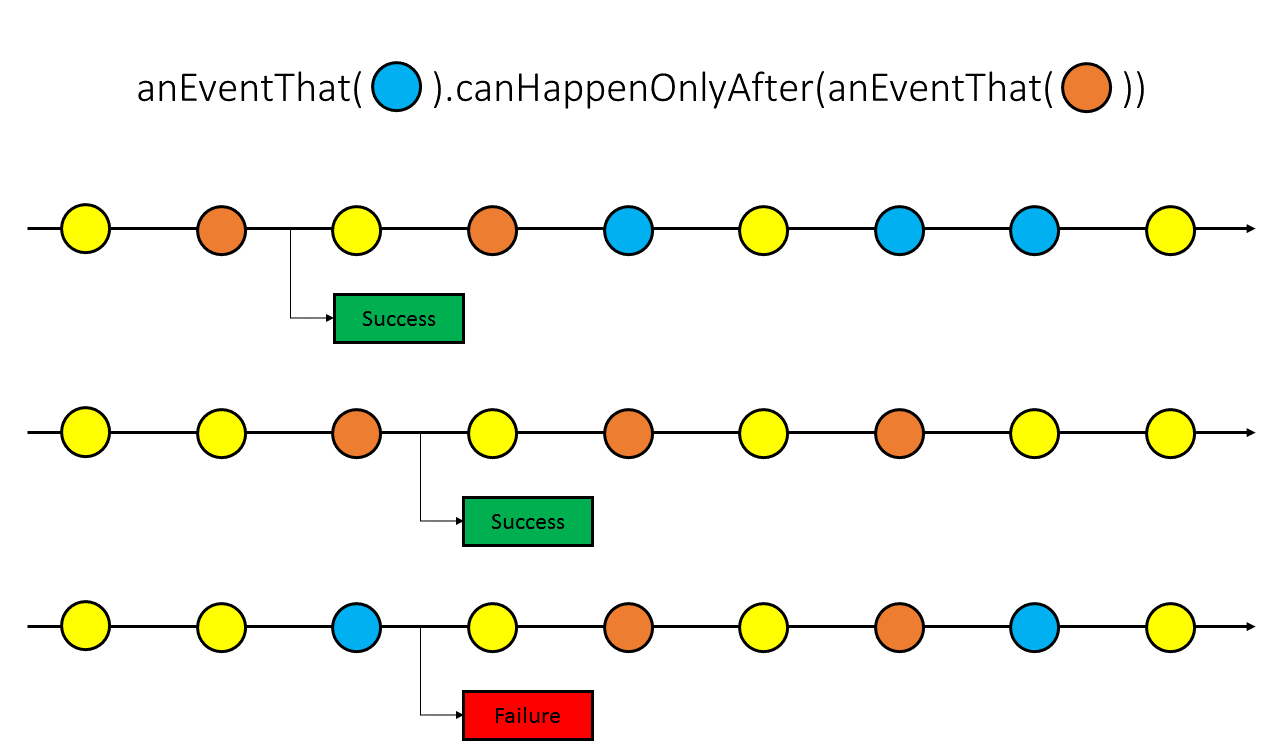
\includegraphics[width=400px]{Images/Language/CanHappenOnlyAfter.png}}
	
	Note in particular that in the second case the checks succeeds even if no blue event occurs: we are  just saying that blue events \textit{can} happen after an orange one.
	
  	\\ \hline
  	
  \rotatebox[origin=c]{90}{\textbf{ Code Example }} & 
  
  	\begin{lstlisting}
	anEventThat(isMarkerPlacement())
		.canHappenOnlyAfter(anEventThat(isMapReady()))
	\end{lstlisting}
	
  	\\ \hline  	
  	 
\end{longtable}
\egroup
\end{center}

\subsection{Checks on Sets of Events}

These checks work on sets of events: for example we may say that a certain event generates a set of \textit{n} other events. The cardinality of each set is specified by the quantifiers
\begin{itemize}
	\item exactly
	\item at most
	\item at least
\end{itemize}
Only the formulas for "exactly" will be written since the others can be derived by analogy.\bigskip \\
First Order Logic specifications use the counting quantifiers~\cite{Pratt-Hartmann:2014:LCE:2603088.2603117} as a notational shorthand, i.e. $\exists_{=n} x$ means that there exist exactly \textit{n} elements \textit{x}.

\subsubsection{Must Happen After}

\begin{center}
\bgroup
\def\arraystretch{1.5}%
\begin{longtable}{ | m{0.3cm} | m{15cm} | }
  \hline
  
  \rotatebox[origin=c]{90}{\textbf{ Structure }} & 
  
  	\begin{lstlisting}
	exactly(n).eventsWhereEach(m1).mustHappenAfter(anEventThat(m2))
	\end{lstlisting}
	
  	\\ \hline
  	 
  \rotatebox[origin=c]{90}{\textbf{ Description }} & 
  
  	Checks that exactly \texttt{n} events that match \texttt{m1} happen exclusively after every event that matches \texttt{m2}. "Exclusively" means that there cannot be another event that matches \texttt{m2} before the sequence of \texttt{n} events is completed.
	
  	\\ \hline

  \rotatebox[origin=c]{90}{\textbf{ FOL }} & 
  
  	\begin{multline*}
	\forall e2 \Bigg( match(e2, m2) \Rightarrow \exists_{=n} e1 \bigg( match(e1, m1) \land before(e2, e1) \\ \land \neg \exists e2' \Big( match(e2', m2) \land between(e2, e2', e1) \Big) \bigg) \Bigg)
	\end{multline*}
	
  	\\ \hline

  \rotatebox[origin=c]{90}{\textbf{ Visual }} & 
  
	\raisebox{-280pt}{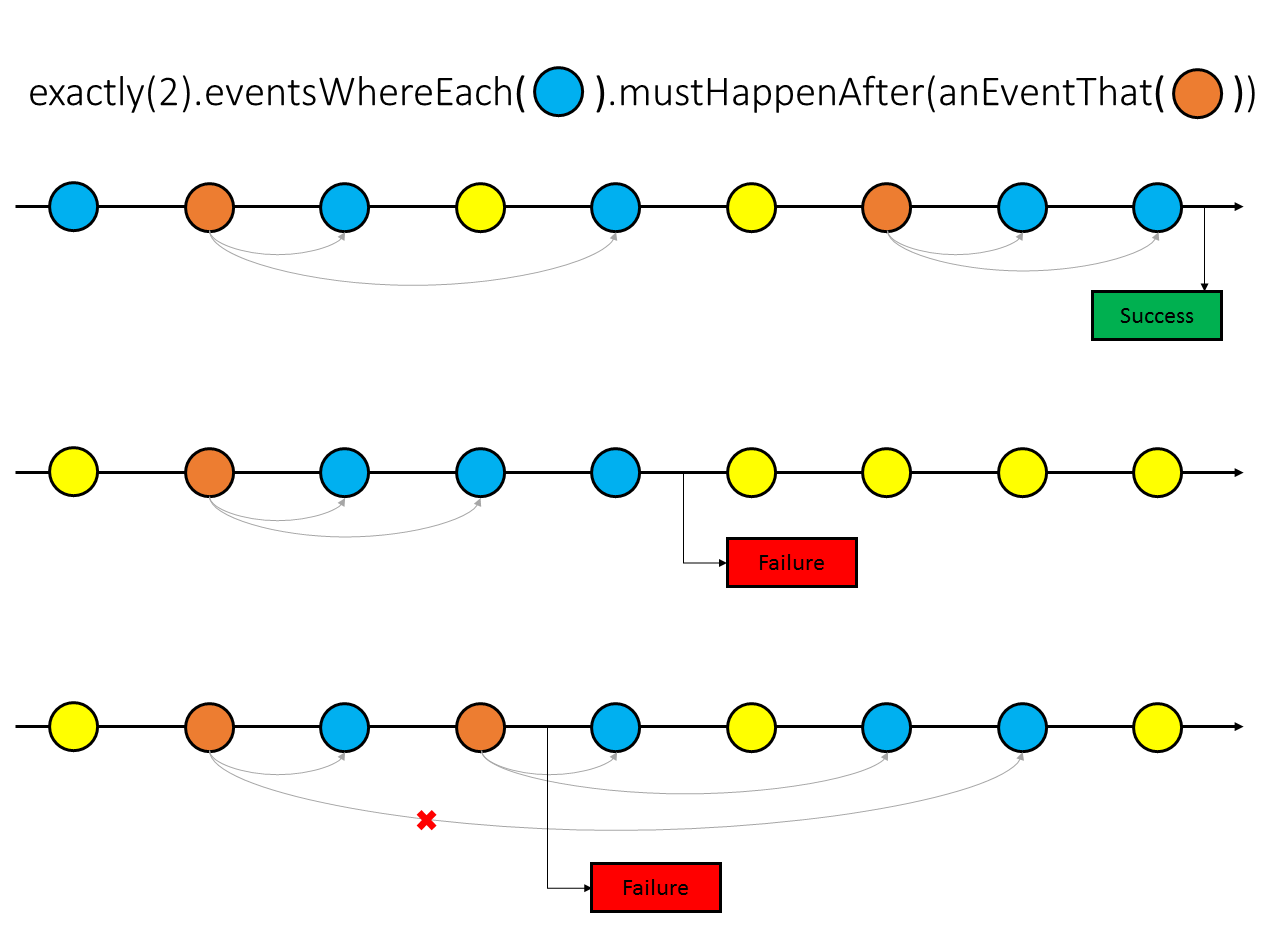
\includegraphics[width=400px]{Images/Language/MustHappenAfter.png}}
	
	Note in particular that the third case shows the "exclusively" constraint mentioned before: the check fails because we do not have two blue events after the first orange but before the second one (i.e. the first orange event does \textit{not} match one of the three blue events that follow the second orange event)

  	\\ \hline
  	
  \rotatebox[origin=c]{90}{\textbf{ Code Example }} & 
  
  	\begin{lstlisting}
	exactly(1).eventsWhereEach(isTextChangeFrom(locationTextView))
		.mustHappenAfter(anEventThat(isLocationChange()))
	\end{lstlisting}
	
  	\\ \hline  	
  	 
\end{longtable}
\egroup
\end{center}

\subsection{Checks on the Whole Stream}

The third type of checks concerns the entire stream of events: they allow for example to specify the number of all the events of a certain type in the whole sequence generated by a particular execution.

\subsection{Connectives between Checks}

These constructs allow to specify the standard logic connectives between one or more of the previously defined consistency checks.

\subsubsection{All Hold}

\begin{center}
\bgroup
\def\arraystretch{1.5}%
\begin{longtable}{ | m{0.3cm} | m{15cm} | }
  \hline
  
  \rotatebox[origin=c]{90}{\textbf{ Structure }} & 
  
  	\begin{lstlisting}
	allHold(c1, c2,...)
	\end{lstlisting}
	
  	\\ \hline
  	 
  \rotatebox[origin=c]{90}{\textbf{ Description }} & 
  
  	All sub-checks \textit{c1}, \textit{c2}, etc. must succeed.
	
  	\\ \hline

  \rotatebox[origin=c]{90}{\textbf{ FOL }} & 
  
  	\begin{multline*}
	c1 \land c2 \land ...
	\end{multline*}
	
  	\\ \hline

  \rotatebox[origin=c]{90}{\textbf{ Visual }} & 
  
	\raisebox{-105pt}{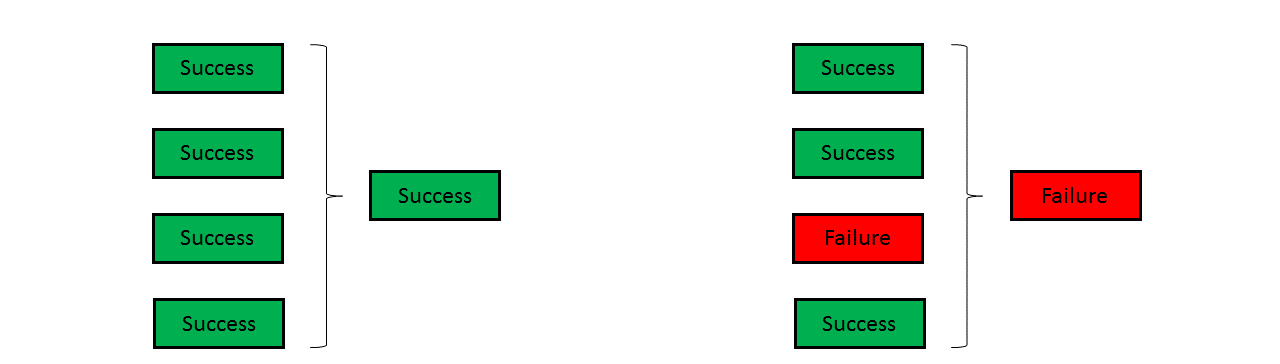
\includegraphics[width=400px]{Images/Language/AllHold.png}}
	
	
  	\\ \hline
  	
  \rotatebox[origin=c]{90}{\textbf{ Code Example }} & 
  
  	\begin{lstlisting}
	allHold(
		exactly(1).eventsWhereEach(isDownloadImage())
			.mustHappenAfter(anEventThat(isClickOn(downloadButton))),
		anEventThat(isEnlargeImage())
			.canHappenOnlyAfter(anEventThat(isDownloadImage)))
	\end{lstlisting}
	
  	\\ \hline  	
  	 
\end{longtable}
\egroup
\end{center}


\section{Design}


\section{Implementation}

For the implementation of event-based testing, the ReactiveX library was chosen. This innovative reactive programming paradigm focuses on data flow: this means generating (statically or dynamically) a flow of events, propagate them and allow interested components to react to them. The idea of reactive programming is fire-and-forget messaging: send a request and asynchronously wait for the response to be ready or, even more importantly, if we are dealing with response sets wait for individual results to be forwarded (without waiting for the whole set to be computed).\bigskip \\
In the next sections a more detailed introduction to the ReactiveX library will be presented, followed by the implementation of the actual event-based testing system.

\subsection{ReactiveX}
The Reactive Extensions (ReactiveX or Rx) are a reactive programming library to compose asynchronous and event-based programs. As defined by its authors, ReactiveX is a combination of the best ideas from
\begin{itemize}
	\item the Observer pattern (design pattern where a subject automatically notifies the so-called observers of its state changes)
	\item the Iterator pattern (design pattern where an iterator is used to traverse a collection of elements, like an array)
	\item functional programming (declarative programming paradigm where computation is performed via mathematical functions that are not allowed to change the state of the system)
\end{itemize}
This approach is asynchronous because many instructions may execute in parallel and their results (events) are later captured, in any order, by the listeners. For this reason, the main idea to perform a computation is not to call methods like in classic sequential programming but to define a mechanism to react to results when they are ready.\bigskip \\
ReactiveX programming paradigm is essentially based on three steps:
\begin{itemize}
	\item Create: the Observable components are used to generate event or data streams
	\item Transform: Operators allow to modify the event streams (e.g. change each event or filter out some of them) and compose them (e.g. join two streams)
	\item Listen: Subscriber components can listen to event streams and receive their elements one by one, to perform some computation
\end{itemize}
An Observable is in charge of emitting events: it generates zero, one or more than one events (depending on the specific implementation), and then terminates either by successfully completing or with an error. Observables can be "hot" (emit events even if no Subscriber is listening) or "cold" (emit events only after a Subscriber is registered).\medskip \\
An Observable can be modified by an Operator: most operators can be applied on an event stream generated by an Observable to return a new modified event stream. For example the operator \texttt{map(function)} allows to apply a function to each event in the stream (e.g. a stream of numbers modified by a map with a summing function may become a stream where all the original numbers have been increased by 1). Since the result of an operator is an Observable, operators can be applied in chain (i.e. apply an operator on the result of another operator) to achieve complex modifications.\medskip \\
A Subscriber consumes the events emitted by the Observables (that can either be "original" or the result of one or more Operators). Subscribers allow to react to asynchronous results: for example, an Observer may send a network response whenever it is ready, the Subscriber receives it and shows the information to the user.\bigskip \\
The advantages of the Rx paradigm are:
\begin{itemize}
	\item Cross-Platform: it is available in many programming languages, like RxJava, RxSwift, RxJS, RxPHP, etc.
	\item Can be used for any application, from Front-End (e.g. UI events and API responses) to Back-End (e.g. asynchronicity and concurrency)
	\item Operators usually make computations less verbose and more readable
	\item Error handling: if an error occurs in one of the steps of the computation the exception is automatically intercepted by Rx and forwarded to the user via appropriate callbacks
	\item Easy concurrency: Rx allows to easily specify in which threads the components should be run, without worrying about implementation details
	\item Extensible: a developer can define custom Observables, Operators and Subscribers to achieve anything an application may require
\end{itemize}
The characteristics of ReactiveX make this programming paradigm very suitable for many applications. It is successfully employed in industry: examples of users of Rx are Microsoft, Netflix and GitHub.

\subsection{RxJava and RxAndroid}
RxJava~\cite{RxJava} is the Java implementation of ReactiveX. It is an open source project initially developed by Netflix for server-side concurrency. The main reason for its adoption and development was to avoid Java Futures (results of asynchronous computation) and callbacks because both are expensive when composed, especially if nested.\smallskip \\
In addition to implementing all functionalities of ReactiveX paradigm (Observables, Subscribers, Operators, etc.), RxJava also has the advantages of being
\begin{itemize}
	\item Lightweight: zero dependencies and single small JAR to contain the whole library
	\item Polyglot: supports Java 6 or higher and JVM-based languages such as Groovy, Clojure, JRuby, Kotlin and Scala
	\item Composable: several RxJava Libraries are available to developers to manage  common use cases
\end{itemize} \bigskip
RxAndroid~\cite{RxAndroid} is a RxJava module that provides specific bindings for the Android platform, for example to easily specify the main (UI) thread as the observing thread or, more in general, a custom Looper. RxAndroid can in turn be extended by other modules, some of which are listed in the next section.

\subsection{Events Observable in Android}
Several modules allow Android developers to observe many events inside an application. For example, we can observe:
\begin{itemize}
	\item UI Widgets: RxBinding~\cite{RxBinding} module allows to observe user inputs or changes on UI widgets like TextView (e.g. clicks, text change), app bar menu (e.g. option selected), etc.
	\item Settings: RxPreferences~\cite{RxPreferences} module allows to receive events from the Shared Preferences system (storage provided by Android to store the app settings)
	\item Files: RxFileObserver~\cite{RxFileObserver} fires events for file accesses or changes
	\item Database: StorIO~\cite{StorIO} allows to manage and observe an SQLite database
	\item Network: ReactiveNetwork~\cite{ReactiveNetwork} detects network changes (e.g. WiFi or mobile connection)
	\item External API Requests: Retrofit~\cite{Retrofit} offers observables to receive network responses (REST client)
	\item Broadcasts: RxBroadcast~\cite{RxBroadcast} builds an event stream from a Broadcast Receiver results
	\item Location: ReactiveLocation~\cite{ReactiveLocation} allows to observe location changes
	\item Sensors: ReactiveSensors~\cite{ReactiveSensors} fires events from hardware sensors
	\item Permissions: RxPermissions~\cite{RxPermissions} allows to receive events from the permissions manager
	\item Google Maps: RxGoogleMaps~\cite{RxGoogleMaps} fires events related to Google Maps
	\item Google Wear: RxWear~\cite{RxWear} allows to observe messages to and from a connected smartwatch
\end{itemize}
And many others.\bigskip \\
The utility module RxLifecycle~\cite{RxLifecycle} allows to bind the listed observables to the lifecycle of an Activity or a Fragment to avoid leaks. For example, without any binding to the lifecycle, an observable that emits text change events on a TextView never ends (i.e. never calls \texttt{onCompleted()} or \texttt{onError()}) because it has no way of understanding when the text will stop changing. In that situation the observable will run even after the Activity has been removed and, keeping its reference, won't allow the garbage collector to delete the instance (memory leak). Thanks to RxLifecycle the developer can bind the observable until a lifecycle event occurs (e.g. activity is stopped), allowing it to terminate correctly.







\section{Evaluation}


%..............................................................................%
%................................. CONCLUSION .................................%
%..............................................................................%

\part{Conclusion}

\section{Recap}

\section{Future Work}


%..............................................................................%
%.................................. REFERENCES ................................%
%..............................................................................%

\bibliographystyle{plain}
\bibliography{Bib/DEvA,Bib/CAFA,Bib/EventRacer,Bib/JUnit,Bib/Lint,Bib/Mockito,Bib/Oracles,Bib/ReactiveLocation,Bib/ReactiveNetwork,Bib/ReactiveSensors,Bib/Retrofit,Bib/Robolectric,Bib/RxAndroid,Bib/RxBinding,Bib/RxBroadcast,Bib/RxFileObserver,Bib/RxGoogleMaps,Bib/RxJava,Bib/RxLifecycle,Bib/RxPermissions,Bib/RxPreferences,Bib/RxWear,Bib/StorIO,Bib/THOR,Bib/CountingLogic} 

\end{document}


